% Figure 1 -- decoder-computation characterization framework.
% Standalone TikZ source (compile: pdflatex figure1_framework.tex) -> figure1_framework.pdf
\documentclass[border=8pt]{standalone}
\usepackage[T1]{fontenc}
\usepackage{helvet}
\renewcommand{\familydefault}{\sfdefault}
\hyphenpenalty=10000 \exhyphenpenalty=10000 \tolerance=2000
\usepackage{amsmath}
\usepackage{tikz}
\usetikzlibrary{arrows.meta, positioning, calc, shadows.blur, fit}

\definecolor{cInk}{HTML}{22303f}
\definecolor{cSub}{HTML}{5c6b7a}
\definecolor{cBlue}{HTML}{34557a}
\definecolor{cTeal}{HTML}{2f7d5f}
\definecolor{cRed}{HTML}{b0413e}
\definecolor{cGold}{HTML}{ab7513}
\definecolor{cLine}{HTML}{b6bec7}
\definecolor{cBlueBg}{HTML}{eef3f8}
\definecolor{cTealBg}{HTML}{ecf5f0}
\definecolor{cRedBg}{HTML}{faeeee}
\definecolor{cGoldBg}{HTML}{f8f1e3}

\tikzset{
  >={Stealth[length=2.6mm,width=2mm]},
  flow/.style={draw=cLine, line width=0.9pt, rounded corners=2.5pt},
  bigarrow/.style={-{Stealth[length=4mm,width=3.6mm]}, draw=cSub, line width=1.6pt},
  card/.style 2 args={draw=#1, line width=1pt, rounded corners=3.5pt, fill=#2,
      inner sep=7pt, align=center, text=cInk,
      blur shadow={shadow blur steps=5, shadow xshift=0.5pt, shadow yshift=-0.8pt, shadow opacity=16}},
  plain/.style={draw=cLine!140, line width=1pt, rounded corners=3.5pt, fill=white,
      inner sep=7pt, align=center, text=cInk,
      blur shadow={shadow blur steps=5, shadow xshift=0.5pt, shadow yshift=-0.8pt, shadow opacity=14}},
  view/.style 2 args={draw=#1, line width=1pt, rounded corners=3.5pt, fill=#2,
      inner sep=8pt, align=left, text=cInk, text width=5.85cm,
      blur shadow={shadow blur steps=5, shadow xshift=0.5pt, shadow yshift=-0.8pt, shadow opacity=16}},
  pill/.style={draw=cLine!140, line width=0.8pt, rounded corners=6pt, fill=white,
      inner sep=3.5pt, font=\footnotesize, text=cSub},
}
\newcommand{\ttl}{\bfseries}
\newcommand{\sub}{\footnotesize\color{cSub}}
\newcommand{\viewtag}[2]{{\footnotesize\scshape\color{#1}#2}}

\begin{document}
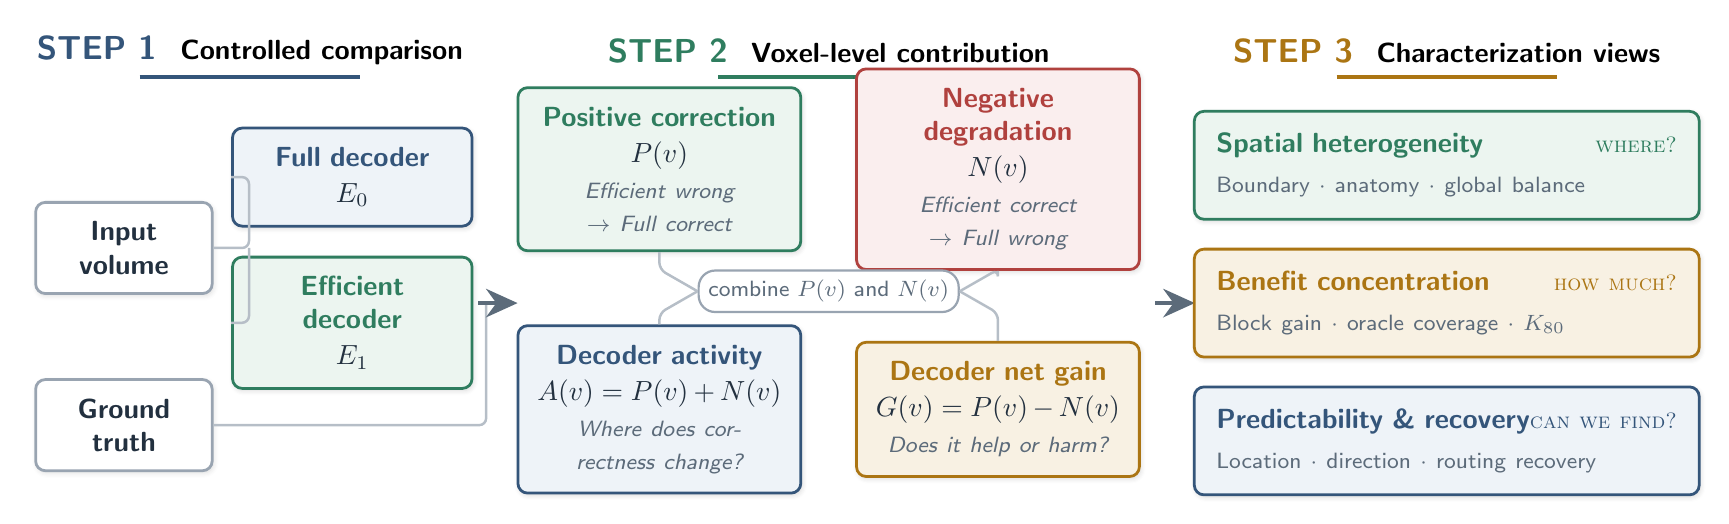
\begin{tikzpicture}

% ===================== STEP headers (centered over each column) =====================
\node[font=\bfseries] at (2.55,5.75) {\textcolor{cBlue}{\large STEP 1}\;\, Controlled comparison};
\node[font=\bfseries] at (9.90,5.75) {\textcolor{cTeal}{\large STEP 2}\;\, Voxel-level contribution};
\node[font=\bfseries] at (17.75,5.75){\textcolor{cGold}{\large STEP 3}\;\, Characterization views};
\draw[cBlue, line width=1.3pt] (1.15,5.42) -- (3.95,5.42);
\draw[cTeal, line width=1.3pt] (8.50,5.42) -- (11.30,5.42);
\draw[cGold, line width=1.3pt] (16.35,5.42) -- (19.15,5.42);

% ===================== STEP 1 =====================
\node[plain, text width=1.75cm] (input) at (0.95,3.25) {\ttl Input\\ volume};
\node[card={cBlue}{cBlueBg}, text width=2.55cm] (e0) at (3.85,4.15)
     {\ttl\textcolor{cBlue}{Full decoder}\\[1pt]\normalfont\itshape $E_0$};
\node[card={cTeal}{cTealBg}, text width=2.55cm] (e1) at (3.85,2.30)
     {\ttl\textcolor{cTeal}{Efficient decoder}\\[1pt]\normalfont\itshape $E_1$};
\node[plain, text width=1.75cm] (gt) at (0.95,1.00) {\ttl Ground\\ truth};

\coordinate (b1) at ($(input.east)+(0.45,0)$);
\draw[flow] (input.east) -- (b1) |- (e0.west);
\draw[flow] (b1) |- (e1.west);
\draw[flow] (gt.east) -| (5.55,2.55);

% arrow into step 2
\draw[bigarrow] (5.45,2.55) -- (5.95,2.55);

% ===================== STEP 2 =====================
\node[card={cTeal}{cTealBg}, text width=3.1cm] (pos) at (7.75,4.25)
     {\ttl\textcolor{cTeal}{Positive correction}\\[1pt]\normalfont\itshape $P(v)$\\[1pt]
      \sub Efficient wrong $\rightarrow$ Full correct};
\node[card={cRed}{cRedBg}, text width=3.1cm] (neg) at (12.05,4.25)
     {\ttl\textcolor{cRed}{Negative degradation}\\[1pt]\normalfont\itshape $N(v)$\\[1pt]
      \sub Efficient correct $\rightarrow$ Full wrong};
\node[pill] (comb) at (9.90,2.70) {combine $P(v)$ and $N(v)$};
\node[card={cBlue}{cBlueBg}, text width=3.1cm] (act) at (7.75,1.20)
     {\ttl\textcolor{cBlue}{Decoder activity}\\[1pt]\normalfont\itshape $A(v)=P(v)+N(v)$\\[1pt]
      \sub Where does correctness change?};
\node[card={cGold}{cGoldBg}, text width=3.1cm] (gain) at (12.05,1.20)
     {\ttl\textcolor{cGold}{Decoder net gain}\\[1pt]\normalfont\itshape $G(v)=P(v)-N(v)$\\[1pt]
      \sub Does it help or harm?};

\draw[flow] (pos.south) -- (pos.south|-comb.north) -- (comb.west);
\draw[flow] (neg.south) -- (neg.south|-comb.north) -- (comb.east);
\draw[flow] (comb.west) -- (act.north|-comb.south) -- (act.north);
\draw[flow] (comb.east) -- (gain.north|-comb.south) -- (gain.north);

% arrow into step 3
\draw[bigarrow] (14.05,2.55) -- (14.55,2.55);

% ===================== STEP 3 =====================
\node[view={cTeal}{cTealBg}] (v1) at (17.75,4.30)
     {{\ttl\textcolor{cTeal}{Spatial heterogeneity}}\hfill\mbox{\viewtag{cTeal}{where?}}\\[2.5pt]
      \sub Boundary $\cdot$ anatomy $\cdot$ global balance};
\node[view={cGold}{cGoldBg}] (v2) at (17.75,2.55)
     {{\ttl\textcolor{cGold}{Benefit concentration}}\hfill\mbox{\viewtag{cGold}{how much?}}\\[2.5pt]
      \sub Block gain $\cdot$ oracle coverage $\cdot$ $K_{80}$};
\node[view={cBlue}{cBlueBg}] (v3) at (17.75,0.80)
     {{\ttl\textcolor{cBlue}{Predictability \& recovery}}\hfill\mbox{\viewtag{cBlue}{can we find?}}\\[2.5pt]
      \sub Location $\cdot$ direction $\cdot$ routing recovery};

\end{tikzpicture}
\end{document}
